\documentclass{beamer}
% \usepackage{animate}
\usepackage{multimedia}

\usepackage{pgfpages}
\setbeameroption{show notes on second screen}
%https://tug.ctan.org/macros/latex/contrib/beamer/doc/beameruserguide.pdf

\usepackage[T2A]{fontenc}
\usepackage[utf8]{inputenc}
\usepackage[english,russian]{babel}
\usepackage{amsmath}
\usepackage{textcomp}
% \usepackage{hyperref}
% \usepackage{bookmark}
\hypersetup{unicode=true}

\setbeamertemplate{caption}[numbered]

\usetheme{CambridgeUS}
\usecolortheme{dolphin}


\title[Отсечение]{Отсечение}
\author[Быковских Д.А.]{Быковских Дмитрий Александрович}
\date{19.10.2024}

\begin{document}
	\begin{frame}
		\titlepage
	\end{frame}

	\begin{frame}{Отсечение}{Clipping}
%eor.dgu.ru/lectures_f/Курс_леций_Компьютерная_геометрия_и_графика_Гаджиев_А_М/лекция_8.htm
		Отсечение – это процесс, связанный с выделением и визуализацией фрагмента плоской или пространственной сцены, расположенного внутри (внутреннее отсечение) или, наоборот, вне (внешнее отсечение) некоторой соответственно двумерной или трехмерной отсекающей фигуры (отсекателя). Оставшаяся часть сцены при этом игнорируется, т.е. визуализации не подлежит.

		Изображение формируется на основе связанных вершин.

		\note{
			На этом этапе могут решаться следующие задачи
			\begin{enumerate}
				\item Визуализация определенной части сцены, т.е. применяется для удаление невидимых линий и поверхностей;
				\item Применение в алгоритмах построения теней.
			\end{enumerate}

			Свойства
			\begin{enumerate}
				\item двумерное или трехмерное;
				\item регулярная (например, прямоугольник, параллелепипед) или нерегулярная структура (отсекатель);
				\item внутреннее и/или внешнее.
			\end{enumerate}
		}
	\end{frame}

	\begin{frame}{Алгритм Коэна и Сазерленда (Cohen-Satherland algorithm)}{Двумерное отсечение}

		Рассматривается случай с параллельными границами, которые также параллельны осям координат.
		\begin{columns}
			\begin{column}{0.4\textwidth}
				\begin{figure} 
					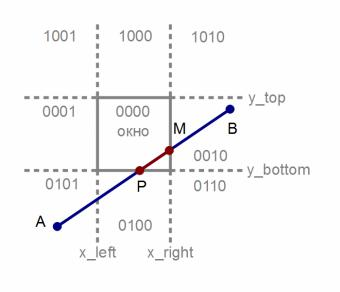
\includegraphics[width=\textwidth]{images/clipping_ex3.jpg}
					\caption{Схема отсечения}
				\end{figure}
			\end{column}
			\begin{column}{0.6\textwidth}
				\centering
				Должно выполняться условие
				$
					\begin{cases}
						x_l \leqslant x \leqslant x_r \\
						y_b \leqslant y \leqslant y_t	\\
					\end{cases}
				$				
				
				\begin{table}
					\caption{таблица кодов}
					\begin{center}
						\begin{tabular}{|c|c|c|}
							\hline
							1001 & 1000 & 1010 \\
							\hline
							0001 & 0000 & 0010 \\
							\hline
							0101 & 0100 & 0110 \\
							\hline
						\end{tabular}
					\end{center}
				\end{table}

				т.е., исходя из условия, определяются бинарные коды, длиной равной 4.
				% (XXXX $\to$ ВНПЛ)
				% Принадлежит или нет.

			\end{column}
		\end{columns}

		\note{
			\hfill Для отрезков получаются следующие коды:
			\begin{columns}
				\begin{column}{0.5\textwidth}
					\begin{figure} 
						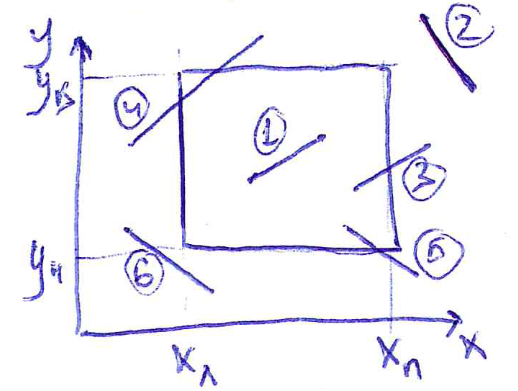
\includegraphics[width=\textwidth]{images/example.png}
						\caption{Схема с различными случаями}
					\end{figure}
				\end{column}
				\begin{column}{0.5\textwidth}
					\begin{enumerate}
						\item 
						$
							\begin{matrix}
								0000 \\
								0000 \\
							\end{matrix}
							= 0000,
						$ виден
						\item 
						$
							\begin{matrix}
								1010 \\
								0010 \\
							\end{matrix}
							= 0010,
						$ не виден
						\item 
						$
							\begin{matrix}
								0000 \\
								0010 \\
							\end{matrix}
							= 0000,
						$ частично виден
						\item 
						$
							\begin{matrix}
								0001 \\
								1000 \\
							\end{matrix}
							= 0000,
						$ частично виден
						\item 
						$
							\begin{matrix}
								0000 \\
								0110 \\
							\end{matrix}
							= 0000,
						$ частично виден
						\item 
						$
							\begin{matrix}
								0001 \\
								0100 \\
							\end{matrix}
							= 0000,
						$ не виден
					\end{enumerate}
				\end{column}
			\end{columns}
		}

	\end{frame}

	
	\begin{frame}{Алгритм Коэна и Сазерленда}{Cohen-Satherland algorithm}


		\begin{figure} 
			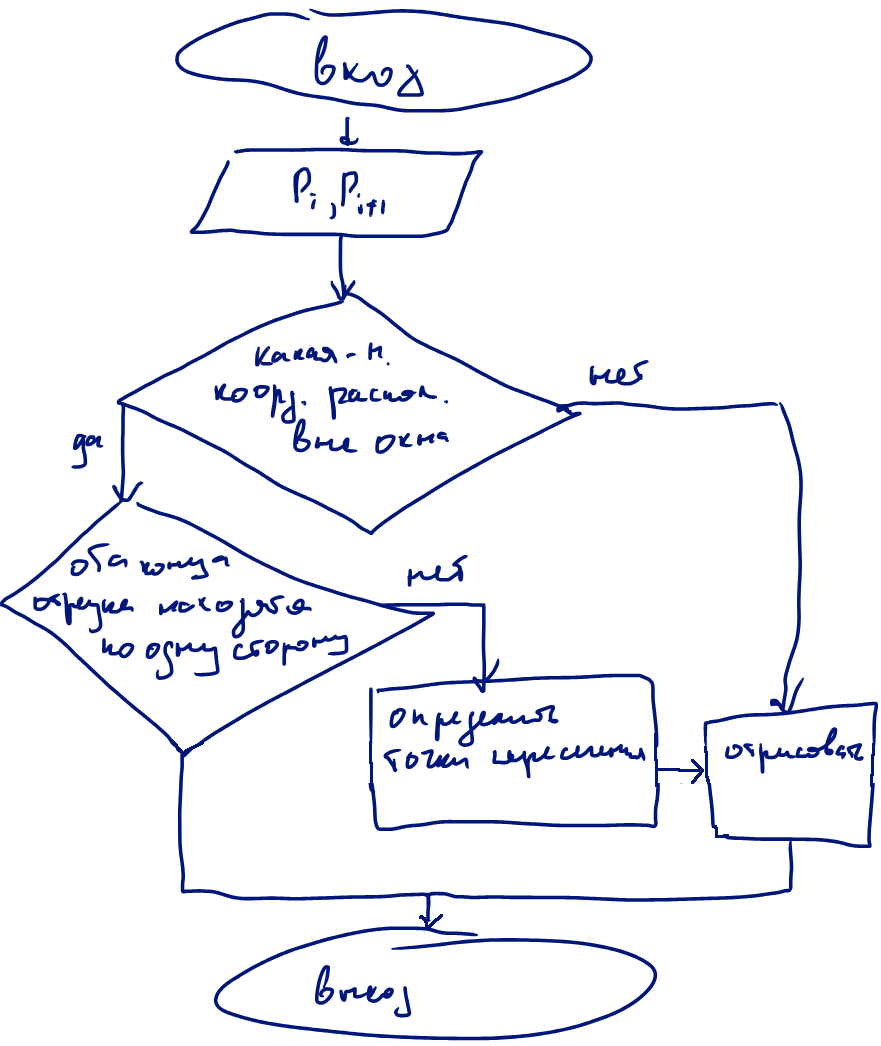
\includegraphics[width=0.42\textwidth]{images/scheme_2d.png}
			\caption{Условный алгоритм двумерного отсечения}
		\end{figure}

		\note{

		}

	\end{frame}

	\begin{frame}{Поиск точки пересечения}

		\begin{columns}
			\begin{column}{0.5\textwidth}

				Рассмотрим задачу пересечения двух отрезков (двух прямых).
				
				Пусть даны координаты отрезка $P_a(x_a, y_a)$ и $P_b(x_b, y_b)$.

				Тогда требуется решить системы уравнений
				\[
					\begin{cases}
						\frac{x - x_a}{x_b - x_a} = \frac{y - y_a}{y_b - y_a}  \\
						\text{уравнение границы}	\\
					\end{cases}
				\]
				
			\end{column}
			\begin{column}{0.5\textwidth}
				\begin{figure} 
					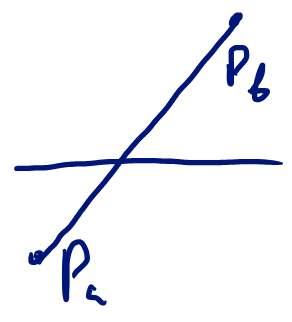
\includegraphics[width=0.6\textwidth]{images/example2.png}
					\caption{Схема пересечения отрезка и отсекателя}
				\end{figure}
			\end{column}
		\end{columns}

		\note{
			Уравнения границ
		\[
			\begin{matrix}
				x = x_l \\
				x = x_r	\\
				y = y_b \\
				y = y_t	\\
			\end{matrix}
		\]
			Определение второй координаты т. пересечения
		\[
			\begin{matrix}
			x_l : y	= y_a + \frac{y_b - y_a}{x_b - x_a}	 (x_l - x_a) \\
			x_r : y	= y_a + \frac{y_b - y_a}{x_b - x_a}	 (x_r - x_a) \\
			y_b : x	= x_a + \frac{x_b - x_a}{y_b - y_a}	 (y_b - y_a) \\
			y_t : x	= x_a + \frac{x_b - x_a}{y_b - y_a} (y_t - y_a) \\
			\end{matrix}
		\]

		При поиске т. пересечения с некоторыми границами отсекателя 
	точки пересечения могут м.б. не обнаружены.
		}

	\end{frame}

	\begin{frame}{Поиск точки пересечения}

		Или может возникнуть следующая проблема...
		\begin{figure} 
			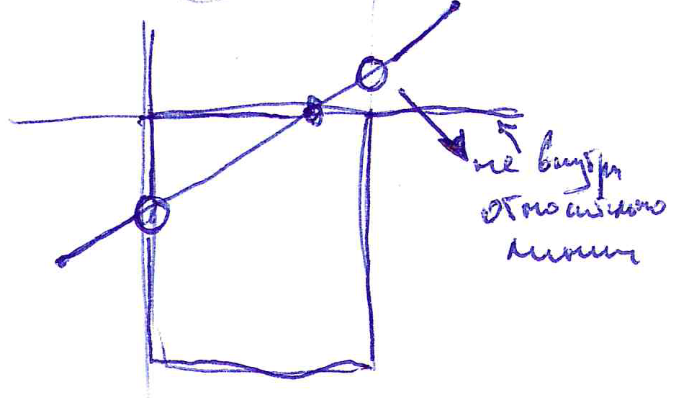
\includegraphics[width=0.65\textwidth]{images/example7.png}
			\caption{Случай пересечения 3х и более точек}
		\end{figure}
		
		\note{
		Примечание.
					Существует также аппаратная реализация, основанная на методе половинного деления отрезка, т.е. побитового свига.

		}

	\end{frame}

	\begin{frame}{Алгоритм Кируса-Бека (Cyrus-Beck)}{Отсечение двумерного отрезка выпуклой областью}

		%Постановка задачи отсечения

		Пусть даны отрезка $P_1$ и $P_2$. 

		Тогда представим в параметрическом виде:

		$P(t) = P_1 + (P_2 - P_1)t$, где $0 \leqslant  t \leqslant 1$

		или можно расписать подробнее:

		\[
		\begin{cases}
			x(t) = x_1 + (x_2 - x_1) t\\
			y(t) = y_1 + (y_2 - y_1) t\\
		\end{cases}	
		\]

		Пусть выпуклая область (окно) задано набором точек $f_j$. Тогда две смежные точки $f_j$ и $f_j+1$ образуют отсекающую линию, у которой можно вычислить нормаль $n_j$.

		\note{
			
			\begin{figure} 
				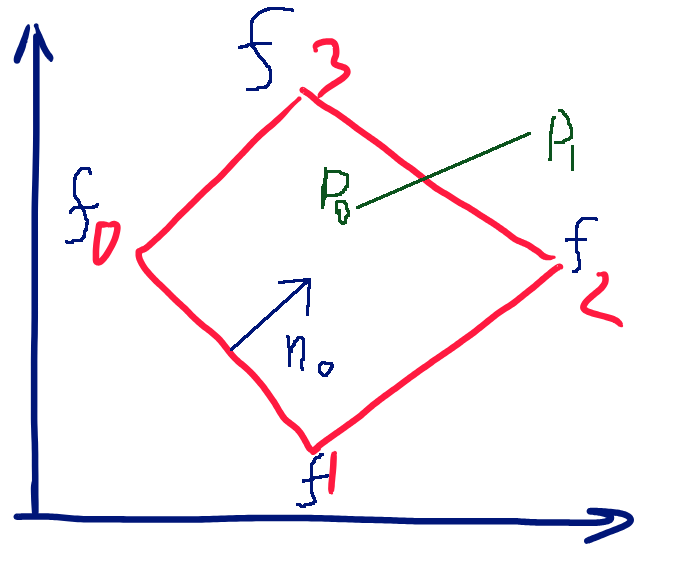
\includegraphics[width=0.6\textwidth]{images/example3.png}
				\caption{Схема}
			\end{figure}
		}
	\end{frame}

	\begin{frame}{Алгоритм Кируса-Бека (Cyrus-Beck)}{Отсечение двумерного отрезка выпуклой областью}
		Для простоты понимания рассмотрим случай плоского выпуклого многоугольника.

		Суть алгоритма заключается в следующем условии
		\[
			n_j [P_i(t) - f_j]
			\begin{cases}
				< 0, & \text{т. находится снаружи, т.к. вектор направлен наружу} \\
				= 0, & \text{т. лежит на границе, т.к. вектор перпендикулярен} \\
				> 0, & \text{т. находится внутри, т.к. вектор направлен внутрь} \\
			\end{cases}
			,
		\]
		где
		$j$ --- номер точки границы;
		$i$ --- номер отрезка;
		$n_j$ --- нормаль границы;
		$f_j$ --- точка выпуклой области;
		$P_i(t)$ --- параметрическое уравнение отрезка.
		
		Примечание. \\ Нормировать вектора необязательно, т.к. интересен только знак.

\note{
Скалярное произведение векторов
\[
	a \cdot b = |a| |b| \cos \theta = a_x b_x + a_y b_y
\]

\begin{figure} 
	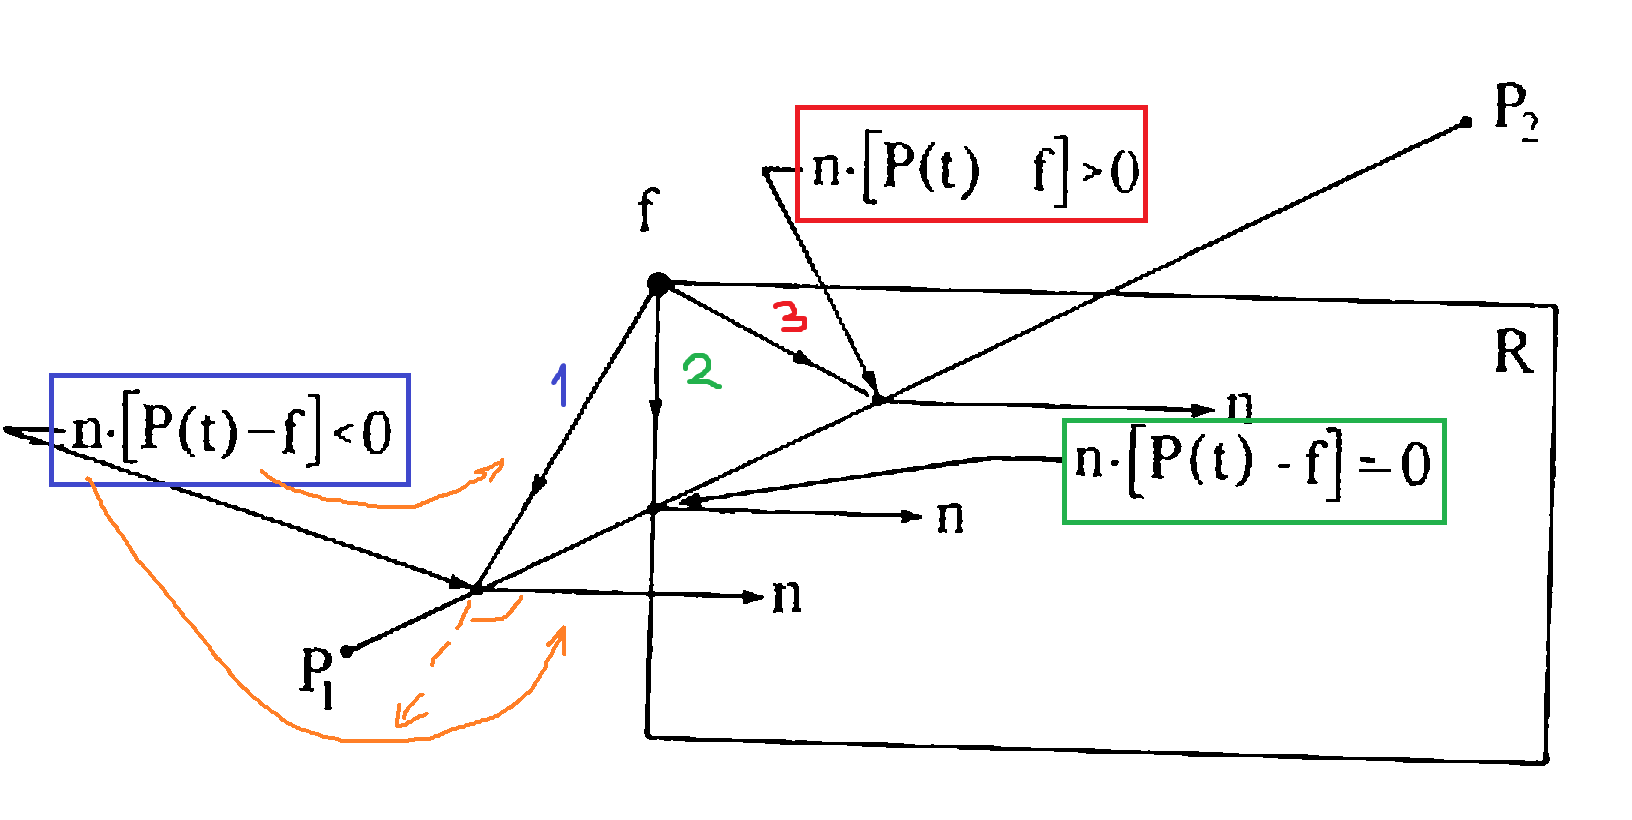
\includegraphics[width=0.8\textwidth]{images/cyrus-beck_scheme.png}
	\caption{Другая схема}
\end{figure}

}
\end{frame}

\begin{frame}{Алгоритм Кируса-Бека (Cyrus-Beck)}{Отсечение двумерного отрезка выпуклой областью}
	Рассмотрим пример.

	\begin{columns}
		\begin{column}{0.5\textwidth}
			Дано: \\
			$P_1(6,-2)$, $P_2(10,1)$. \\
			$F_1(0,0)$, $F_2(8,4)$.
			\\
			Найти: 
			\\
			точку пересечения
			\\
			Решение:
			\\
			Составим параметрическое уравнение отрезка
			\[
				\begin{cases}
					x(t) = 6 + (10 - 6) t\\
					y(t) = -2 + (1 + 2) t\\
				\end{cases}	
			\]
		\end{column}
		\begin{column}{0.5\textwidth}
			\begin{figure} 
				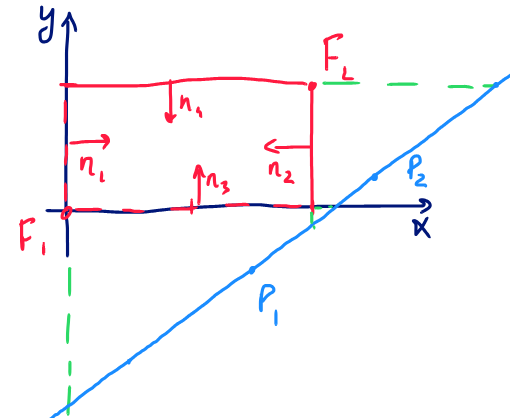
\includegraphics[width=0.9\textwidth]{images/example_cyrus-beck.png}
				\caption {Иллюстрация к примеру}
			\end{figure}
		\end{column}
	\end{columns}





	\note{

	\begin{table}
		% \caption{Пример расчета}
		\begin{center}
			\begin{tabular}{|c|c|c|c|c|c|c|c|}
				\hline
				№ & $n_j$ & $F_j$ & $P_i(t) - F_j$ & $n_j \cdot (P_i(t) - F_j)$ & $t$ \\
				\hline
				$1$ & $(1,0)$ & $(0,0)$ &$(6t+4, -2+3t)$ & $(6t+4)$ & $-3/2$ \\
				\hline
				$2$ & $(-1,0)$ & $(8,4)$ & $(-2t+4, -6+3t)$ & $2t-4$ & $1/2$ \\
				\hline
				$3$ & $(0,1)$ & $(0,0)$ & $(6t+4, -2+3t)$ & $-2+3t$ & $2/3$ \\
				\hline
				$4$ & $(0,-1)$ & $(8,4)$ & $(-2t+4, -6+3t)$ & $6-3t$ & $2$ \\
				\hline
			\end{tabular}
		\end{center}
	\end{table}

	\begin{table}
		% \caption{Пример расчета}
		\begin{center}
			\begin{tabular}{|c|c|c|c|}
				\hline
				№ & $n_j \cdot (P_i(t) - F_j)$ & $t = 1/2$ & $ t = 2/3 $ \\
				\hline
				$1$ & $(6t+4)$ & $8$ & $>0$ \\
				\hline
				$2$ & $2t-4$ & $0$ & $<0$ \\
				\hline
				$3$ & $-2+3t$ & $-0.5$ & \\
				\hline
				$4$ & $6-3t$ & &  \\
				\hline
			\end{tabular}
		\end{center}
	\end{table}

	\footnotesize
	Параметр $t$ должен принадлежать отрезку $[0,1]$.
	
	Поэтому отбрасываются случаи $t = -3/2$ и $t = 2$.

	Далее при подстановке каждого значения параметра $t$ в каждое уравнение скалярное произведение не должно быть отрицательным.
	\\
	-
}
\end{frame}

\begin{frame}{Выпуклость многоугольника}
	Как определить выпуклость многоугольника?

	Для этого используется псевдоскалярное произведение нормалей смежных граней
	\[
		n_i \lor n_{i+1}
		=
		\begin{vmatrix} n_{x,i} & n_{y,i} \\ n_{x,i+1} & n_{y,i+1} \end{vmatrix}
	\]

	При обходе против часовой стрелки
	\[
		n_i \lor n_{i+1}
		\begin{cases}
			\geqslant	0, & \text{выпуклый} \\
			<	0, & \text{вогнутый} \\
		\end{cases}
	\]
	Аналогичным образом формулируется по часовой стрелки при этом знаки меняются наоборот.

	\note{
		\begin{figure} 
			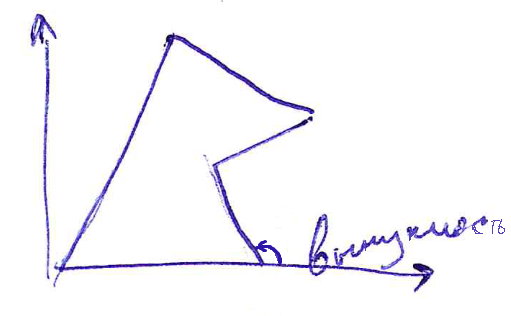
\includegraphics[width=0.45\textwidth]{images/example4.png}
			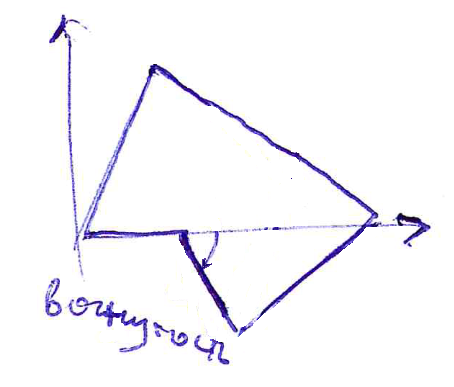
\includegraphics[width=0.38\textwidth]{images/example5.png}
			\caption {Пример определения вогнутой области}
		\end{figure}
		Примечание. \\
		Для таких областей тоже можно строить, но нужно их разбивать на выпуклые области.

	}
	\end{frame}

	\begin{frame}{Трехмерное отсечение}{ для параллелепипеда}
		
		\begin{columns}
			\begin{column}{0.5\textwidth}
				Представленный алгоритм Коэна-Сазерленда можно легко адаптировать для трехмерного случая, расширив кодовую бинарную последовательность для точки до 6 бит.
			\end{column}
			\begin{column}{0.5\textwidth}
				\begin{figure} 
					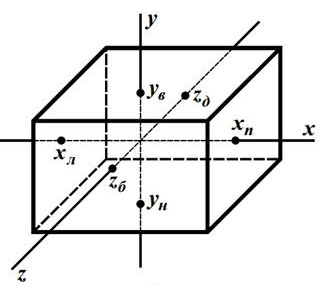
\includegraphics[width=1.0\textwidth]{images/clipping_1.jpg}
					\caption {Прямоугольный параллелепипед}
				\end{figure}
		\end{column}
	\end{columns}





		\note{

		Для точек отрезов $P_i(x,y,z)$, рисуемых на экране, должно выполняться следующее условие:

		\[
			\begin{cases}
				x_l \leqslant x \leqslant x_r \\
				y_b \leqslant y \leqslant y_t	\\
				z_n \leqslant z \leqslant z_f	\\
			\end{cases}
		\]
		}

	\end{frame}

	\begin{frame}{Трехмерное отсечение}{для усеченной пирамиды}

		\begin{columns}
			\begin{column}{0.5\textwidth}
				Рассмотрим трехмерное отсечение для усеченной пирамиды. 

			Каноническая форма: \\
			$x_l = -1$, $x_r = 1$, \\
			$y_b = -1$, $y_t = 1$, \\
			$z_n = a$, $z_f = 1$, \\
			$z_c = 0$,
			\\ где  $0<a<1$.
			\end{column}
			\begin{column}{0.5\textwidth}
		\begin{figure} 
			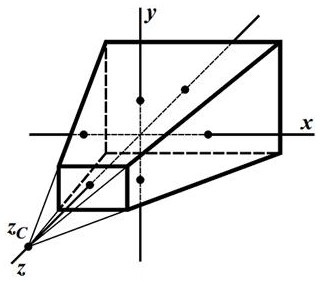
\includegraphics[width=\textwidth]{images/clipping_2.jpg}
			\caption {Усеченная пирамида}
		\end{figure}

		\end{column}
	\end{columns}

	\note{
		Этот вариант актуален для перспективного проецирования.
	}

	\end{frame}
	
	\begin{frame}{Трехмерное отсечение}{}
		\begin{columns}
			\begin{column}{0.5\textwidth}
				\[
					x = \frac{z - z_c}{z_f - z_c} x_r = z \alpha_1 + \alpha_2
					,
				\]
				где 
					$\alpha_1 = \frac{x_r}{z_f - z_c}$,
					$\alpha_2 = - \alpha_1 z_c$.
					
			\end{column}
			\begin{column}{0.5\textwidth}
				\begin{figure} 
					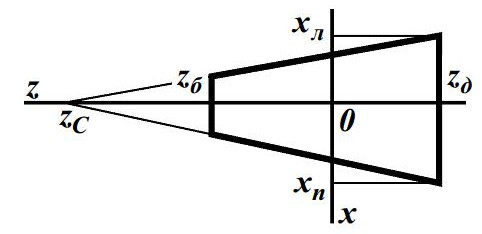
\includegraphics[width=\textwidth]{images/clipping_3.jpg}
					\caption {Проекции вида сверху пирамиды}
				\end{figure}
			\end{column}
		\end{columns}


	\note{
		\[					
			f_r = x - z \alpha_1 - \alpha_2	
			\begin{cases}
				>0, & \text{точка расположена правее плоскости отсечения} \\
				=0, & \text{точка принадлежит плоскости отсечения} \\
				<0, & \text{точка расположена левее плоскости отсечения} \\
			\end{cases}
			,
		\]
		где 
		$\alpha_1 = \frac{x_r}{z_f - z_c}$,
		$\alpha_2 = - \alpha_1 z_c$.

		\[					
			f_l = x - z \beta_1 - \beta_2	
			\begin{cases}
				>0, & \text{точка расположена правее плоскости отсечения} \\
				=0, & \text{точка принадлежит плоскости отсечения} \\
				<0, & \text{точка расположена левее плоскости отсечения} \\
			\end{cases}
			,
		\]
		где 
		$\beta_1 = \frac{x_l}{z_f - z_c}$,
		$\beta_2 = - \beta_1 z_c$.



	}
	\end{frame}
	\begin{frame}{Трехмерное отсечение усеченной пирамиды}

		\begin{figure} 
			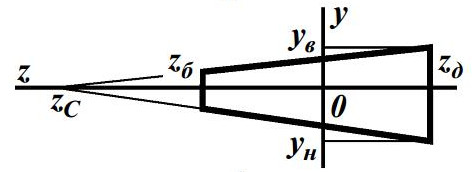
\includegraphics[width=0.8\textwidth]{images/clipping_4.jpg}
			\caption {Проекции вида сбоку пирамиды}
		\end{figure}
		\note{
			\[					
				f_t = y - z \gamma_1 - \gamma_2	
				\begin{cases}
					>0, & \text{точка расположена выше плоскости отсечения} \\
					=0, & \text{точка принадлежит плоскости отсечения} \\
					<0, & \text{точка расположена ниже плоскости отсечения} \\
				\end{cases}
				,
			\]
			где 
			$\gamma_1 = \frac{y_t}{z_f - z_c}$,
			$\gamma_2 = - \gamma_1 z_c$.
	
			\[					
				f_b = y - z \delta_1 - \delta_2	
				\begin{cases}
					>0, & \text{точка расположена выше плоскости отсечения} \\
					=0, & \text{точка принадлежит плоскости отсечения} \\
					<0, & \text{точка расположена ниже плоскости отсечения} \\
				\end{cases}
				,
			\]
			где 
			$\delta_1 = \frac{y_b}{z_f - z_c}$,
			$\delta_2 = - \delta_1 z_c$.
		}
	\end{frame}
	\begin{frame}{Трехмерное отсечение усеченной пирамиды}
		\begin{figure} 
			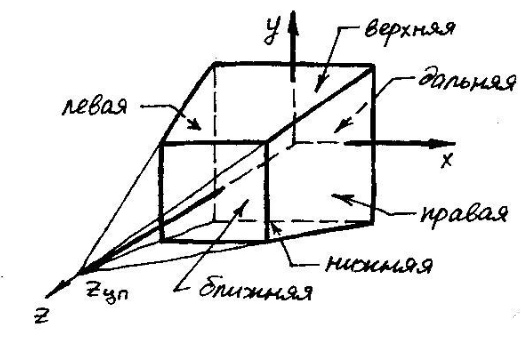
\includegraphics[width=0.8\textwidth]{images/clipping_5.jpg}
			\caption {Проекции вида сбоку пирамиды}
		\end{figure}
		\note{
			\[					
				f_n = z - z_n 
				\begin{cases}
					>0, & \text{точка расположена перед плоскостью отсечения} \\
					=0, & \text{точка принадлежит плоскости отсечения} \\
					<0, & \text{точка расположена за плоскостью отсечения} \\
				\end{cases}
				.
			\]
			\[					
				f_f = z - z_f
				\begin{cases}
					>0, & \text{точка расположена перед плоскостью отсечения} \\
					=0, & \text{точка принадлежит плоскости отсечения} \\
					<0, & \text{точка расположена за плоскостью отсечения} \\
				\end{cases}
				.
			\]
		}
	\end{frame}

	\begin{frame}{Комбинированное отсечение}

		Задачи внутреннего отсечения легко адаптировать к решению задач внешнего отсечения.
		
		
		Результаты внешнего отсечения могут быть получены путем инвертирования (обращения) результатов внутреннего отсечения:
		\begin{itemize}
			\item 
			отрезки или их части, которые при внутреннем отсечении определяются как видимые, при внешнем отсечении на экран не выводятся, 
			\item 
			и, наоборот, отрезки или их части, которые алгоритмом внутреннего отсечения игнорируются, при внешнем отсечении идентифицируются как видимые и визуализируются. 
		\end{itemize}
		
		Комбинированное отсечение --- комбинация внутреннего и внешнего отсечений.

		
		Комбинированное отсечение позволяет реализовать также внутреннее или внешнее отсечение графических объектов невыпуклыми (частично вогнутыми) отсекателями.
		


		\note{
			\begin{columns}
				\begin{column}{0.5\textwidth}
					Характерный пример комбинированного отсечения наблюдается на экране компьютерного дисплея при многооконном режиме его работы под управлением операционной системы.
		
					Содержимое рабочей области пассивного окна 3 подвергается внутреннему отсечению прямоугольником, образованным границами этой области; само окно 3 со всем содержимым подвергается внешнему отсечению окнами 1 и 2, имеющими приоритеты выше, чем окно 3.
				\end{column}
				\begin{column}{0.5\textwidth}
					\begin{figure} 
						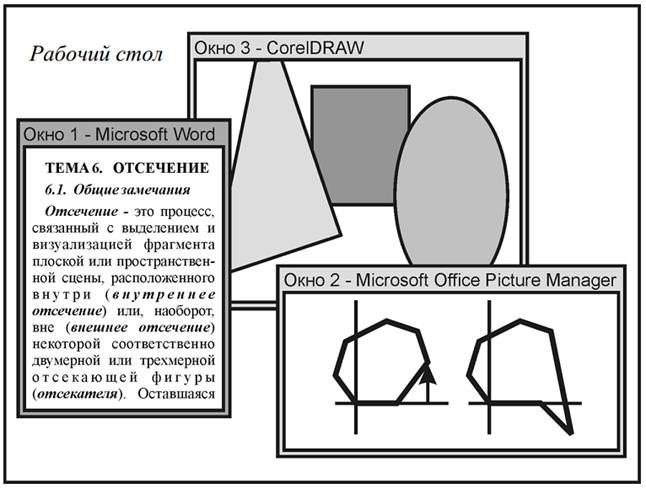
\includegraphics[width=\textwidth]{images/combined_clipping.jpg}
						\caption {Многооконный режим работы}
					\end{figure}
				\end{column}
			\end{columns}

		}
	\end{frame}

	\end{document}
	
	% https://learnwebgl.brown37.net/08_projections/projections_ortho.html
	% https://www.songho.ca/opengl/gl_projectionmatrix.html
	% https://www.scratchapixel.com/lessons/3d-basic-rendering/perspective-and-orthographic-projection-matrix/opengl-perspective-projection-matrix.html
	% https://en.wikipedia.org/wiki/Viewing_frustum
	% https://www.reddit.com/r/opengl/comments/2hs6cf/questionglmfrustum_or_glmperspective/
	% https://startandroid.ru/ru/uroki/vse-uroki-spiskom/401-urok-172-perspective-frustum-ortho.html
	% http://doc.51windows.net/Directx9_SDK/graphics/programmingguide/fixedfunction/viewportsclipping/viewingfrustum.htm
	% https://www.google.com/search?q=camera+transformation+FOV&tbm=isch&ved=2ahUKEwjh6-yX7_CBAxXwBxAIHS7gDtwQ2-cCegQIABAA&oq=camera+transformation+FOV&gs_lcp=CgNpbWcQAzoHCAAQigUQQzoFCAAQgAQ6BggAEAgQHjoHCAAQGBCABDoECAAQHlDSAlizDWDWDmgBcAB4AIABUYgBwwKSAQE2mAEAoAEBqgELZ3dzLXdpei1pbWfAAQE&sclient=img&ei=mxYoZaGyMvCPwPAPrsC74A0&bih=921&biw=1920#imgrc=1JjqcwhhFgAhiM


	\begin{figure} 
		\href{https://www.researchgate.net/figure/Outline-of-the-graphics-pipeline_fig1_281810652}{
			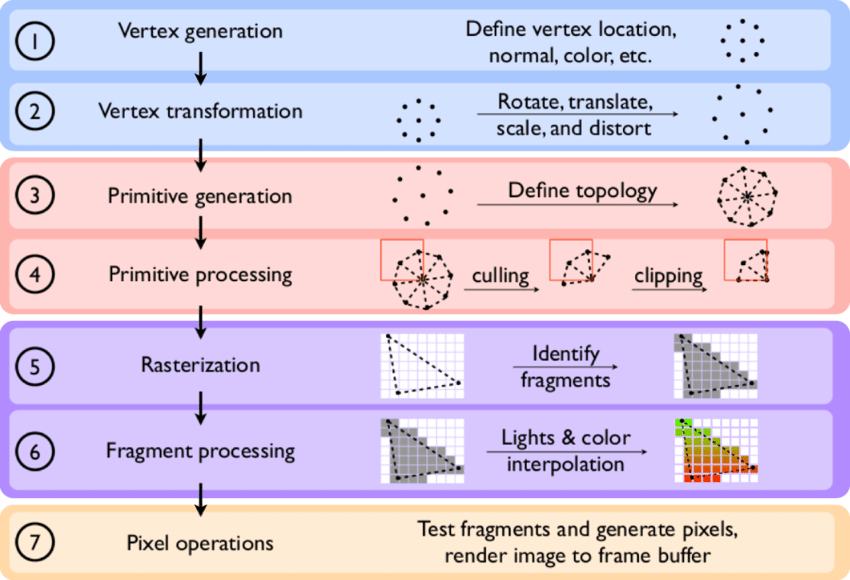
\includegraphics[width=0.75\textwidth]{images/Outline-of-the-graphics-pipeline.png}}
		\caption{Схема графического конвейера}
	\end{figure}

	\begin{figure} 
			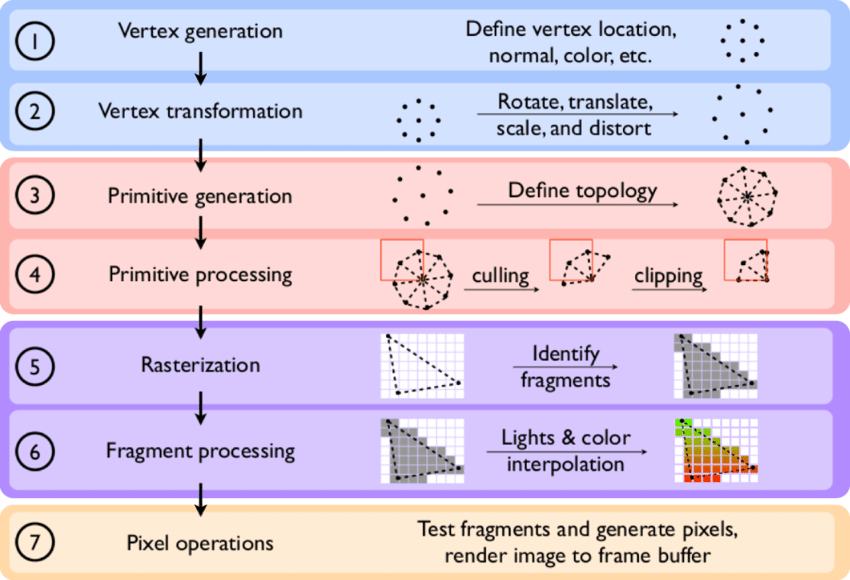
\includegraphics[width=0.75\textwidth]{images/Outline-of-the-graphics-pipeline.png}
		\caption{Схема графического конвейера}
	\end{figure}

	\begin{columns}
		\begin{column}{0.5\textwidth}
			\begin{figure} 
				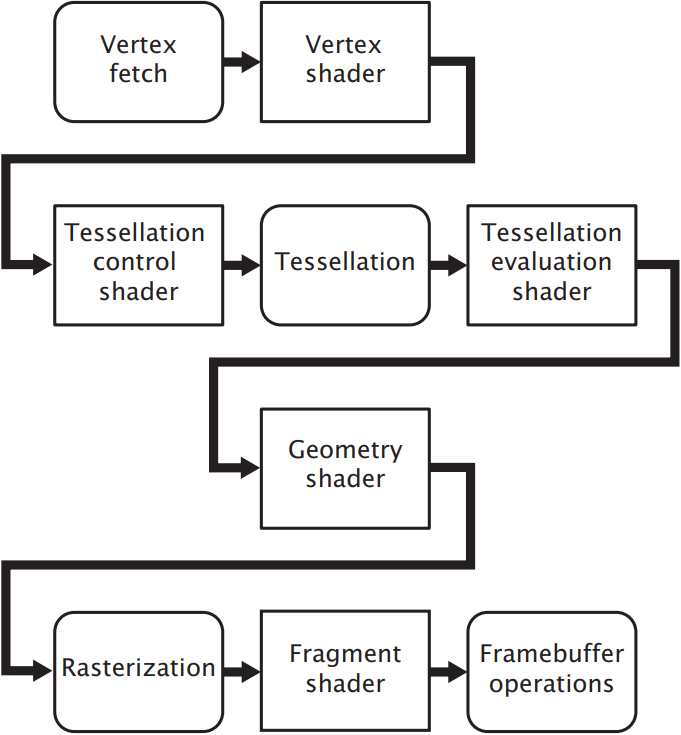
\includegraphics[width=0.9\textwidth]{images/Simplified_model_of_the_graphics_pipeline.png}
				\caption {Порядок вычисления шейдеров}
			\end{figure}
		\end{column}
		\begin{column}{0.5\textwidth}
		\end{column}
	\end{columns}
			

			\footnotesize

			\begin{table}
				% \caption{\label{tab:fractal} Название}
				\begin{center}
					\begin{tabular}{|c|c|c|}
						\hline
						$k$ & $l$ & $N(l)$ \\
						\hline
						0 & $1$ & $1$ \\
						\hline
						1 & $1/2$ & $3$ \\
						\hline
						2 & $1/4$ & $9$ \\
						\hline
						\multicolumn{3}{|c|} {\dots} \\
						\hline
						n & $2^{-n}$ & $3^{n}$ \\
						\hline
					\end{tabular}
				\end{center}
			\end{table}